\section{Introduction}

The Salomon Islands are located in the central Indian Ocean (~5\degree 19' 0'' S, 72\degree 15' 36'' E) approximately 320 nautical miles south of the equator (Figure \ref{Chagos_fig1}). They collectively delimit the borders of one of the atolls of the Chagos Archipelago and provide shelter to the few yachts crossing the Indian Ocean, which, if granted a permit, may anchor in the pristine waters of the lagoon. After the forced relocation of the native Chagossian people, Chagos Archipelago has remained uninhabited except for British and American military personnel located on Diego Garcia, more than 100 nautical miles south of Salomon. The Chagos Archipelago has now become the British Indian Ocean Territory (BIOT), which comprises seven atolls and over 1000 islands spread over approximately 640,000 square kilometers. BIOT was established as a marine protected area in 2010, banning extraction activity and doubling the size of the no-take zones worldwide.

\begin{figure}
    \centering
    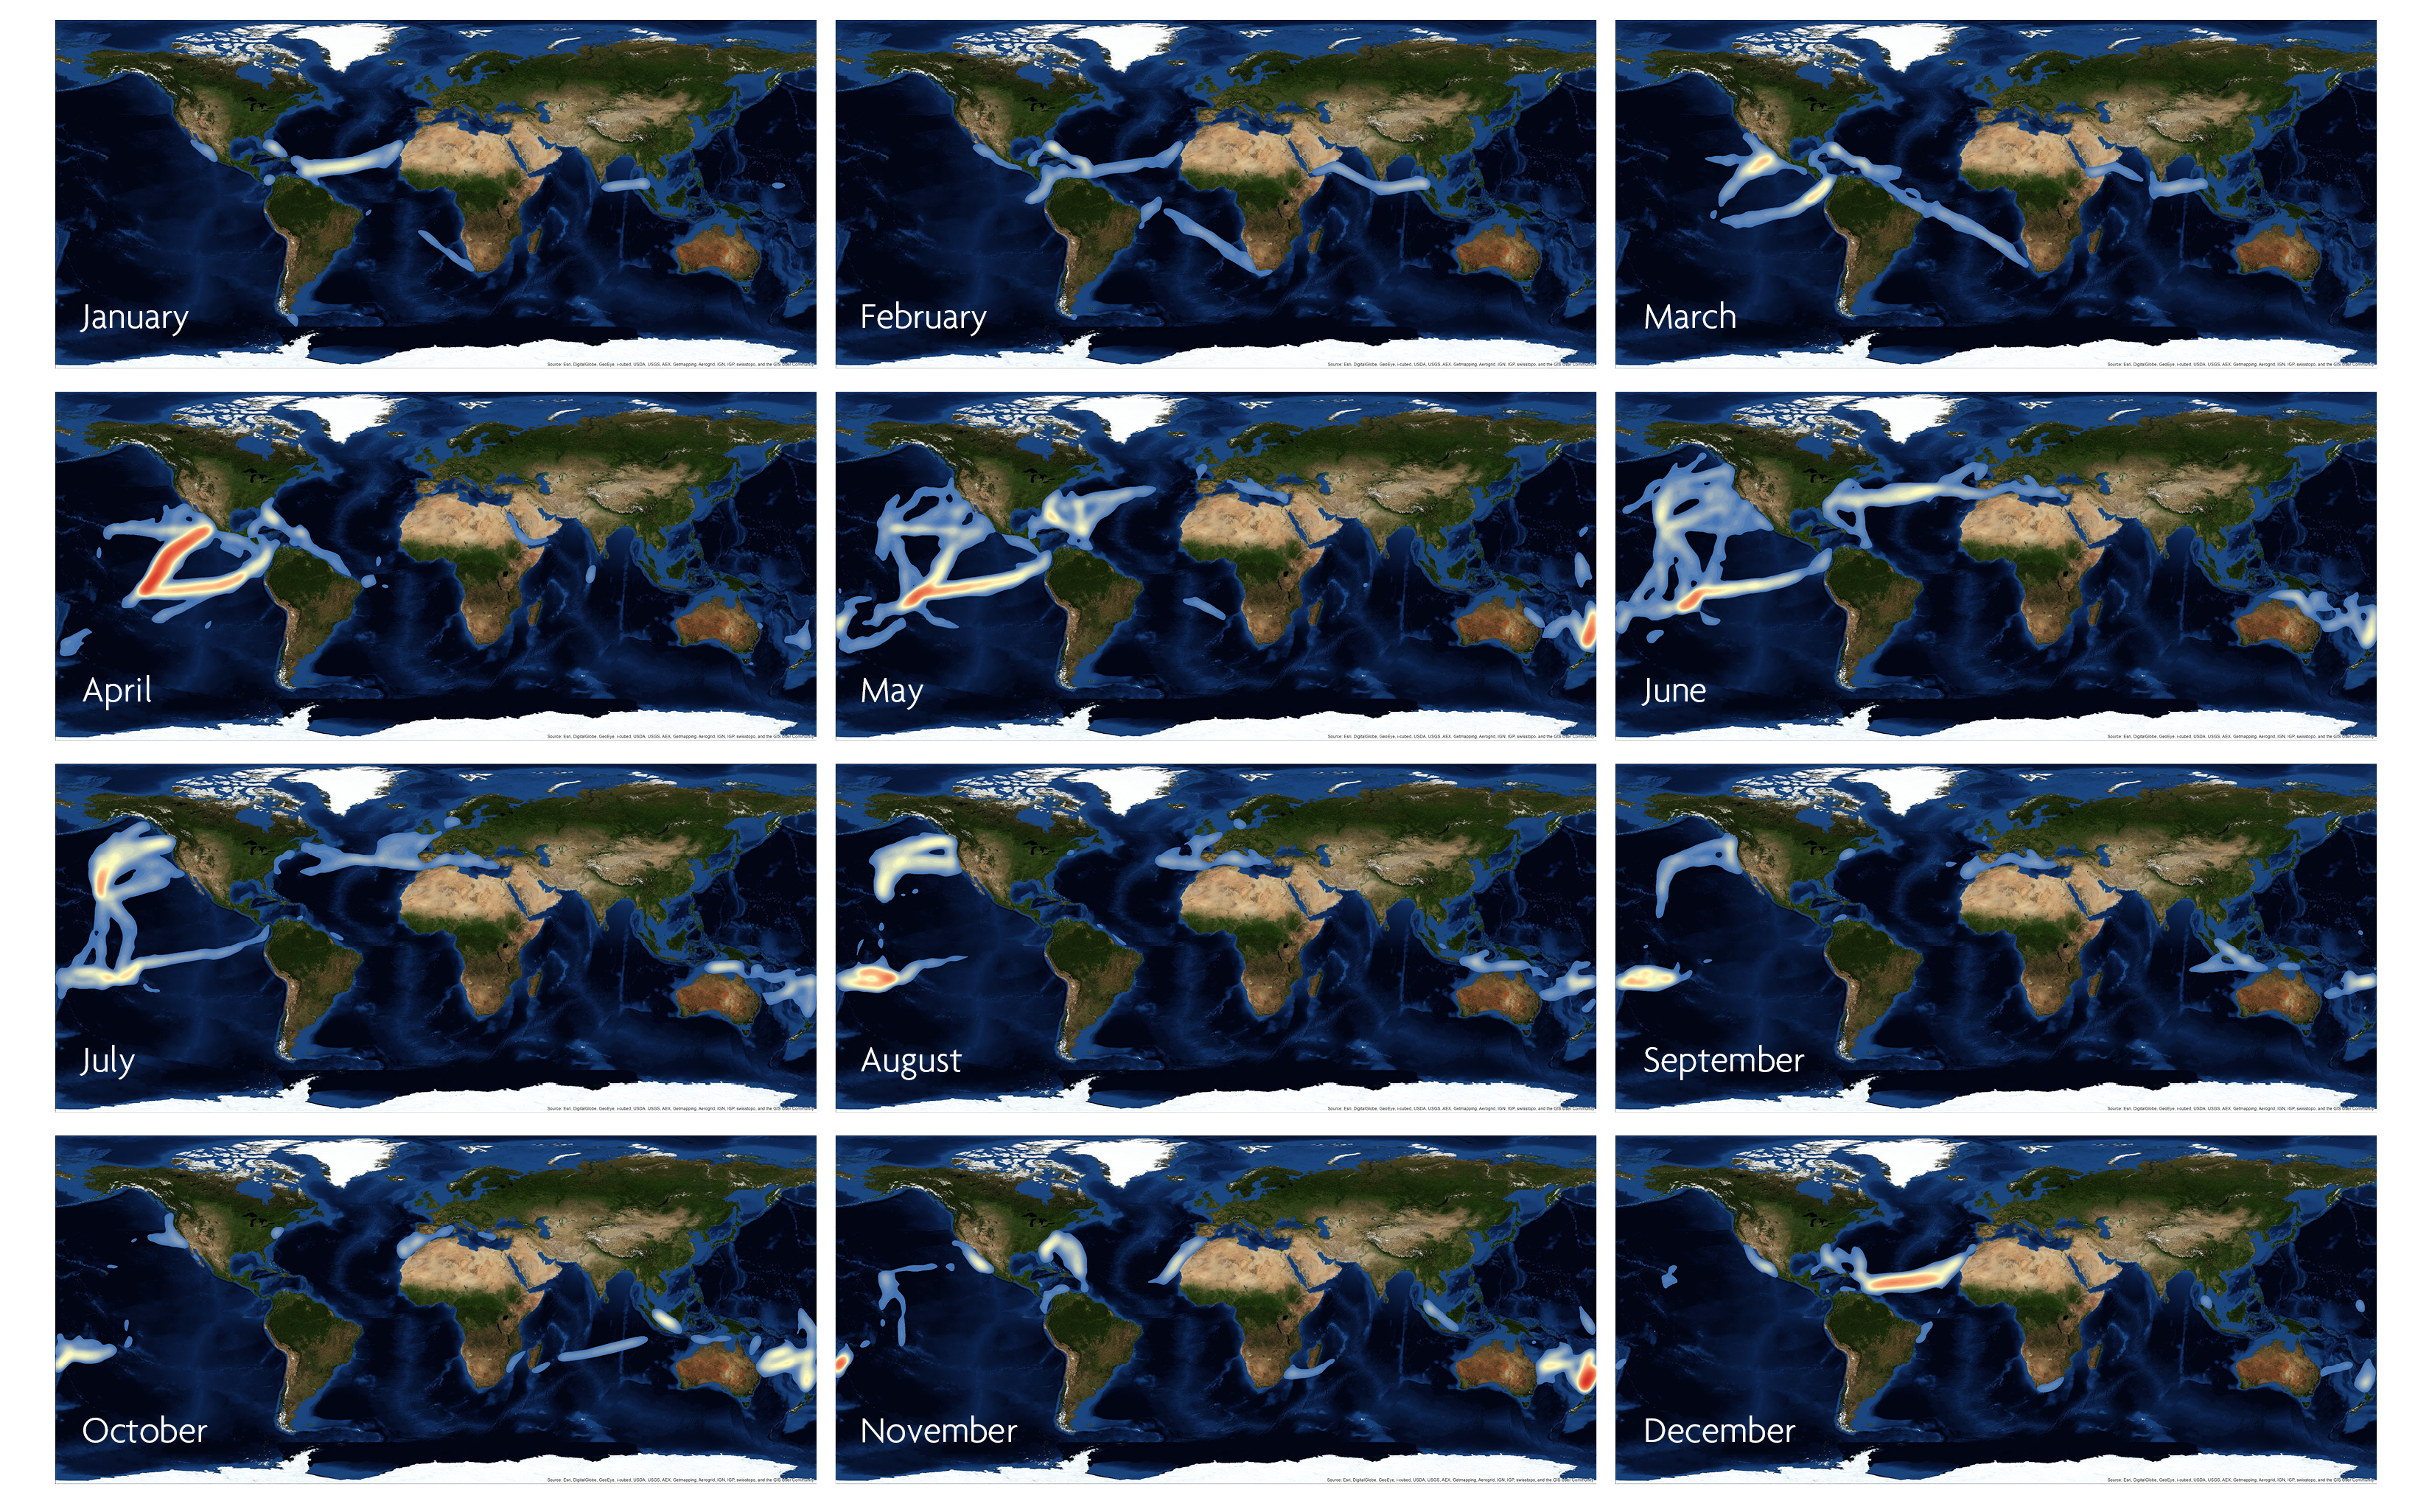
\includegraphics{Chagos/figures/fig1}
    \caption{The chlorophyll concentration of each sample was estimated from MODIS data using ESRI's ArcGIS 10.3 Desktop as described in the methods.}
    \label{Chagos_fig1}
\end{figure}

